\vspace{-.25in}
\section{COMPUTATIONAL READINESS} % typically about 5 pages
\vspace{-.2in}

The proposed simulations will be performed using a GPU-oriented version of
Nek5000, which is a highly scalable open-source code for fluid-thermal
simulation and a Gordon Bell and RD 100 Prize winner \cite{tufo99a}.  This new
code, NekRS, is based on high-performance kernels from the libParanumal library
out of the Warburton group at Viginia Tech
\cite{ChalmersKarakusAustinSwirydowiczWarburton2020,streamParanumal2020} and is
written in the open concurrent computed abstraction (OCCA) for platform
portability \cite{occa}.  NekRS, libParanumal, and OCCA are being developed as
part of DOE's Exascale Computing Project
 in the Center for Efficient Exascale Discretizations (CEED).

\vspace{-.25in}
\subsection{Usage of Resources Requested }
\label{sec:usage2}
\vspace{-.2in}

\noindent{\bf Challenge 1.}
A single SMR assembly with mixing vanes explicitly modeled is expected to
involve approximately 170 million elements. This estimate is based on the work
of Busco et. al. \cite{busco2019invariant} for a 5$\times$5 bundle and extrapolating
to five 17$\times$17 axial grids or roughly $60 \times$ larger.
%
Therefore the first simulation on Summit will aim for 270 million elements (1
assembly modeled explicitly) with the rest of the full core modeled with RANS
(using the mesh of Fang which comprises 100  million elements \cite{Fang2021}).
In the second year we follow with 1.6 billion elements (9 assemblies modeled
explicitly).  Finally in the third year, we perform a 37 assembly simulation
comprising 6.3 billion elements.
%
Using testing performed on Summit with the case of Busco
\cite{nekrs} at $N=7$ we estimate that to advance the full-core mesh
with 1 assembly modeled explicitly on 3420 nodes on Summit will require 0.275s
per time step. We also estimate that 500,000 time steps will be required to
reach statistical convergence based on past experience. This will translate in
130,000 node-hours for the first year on Summit. We note that this calculation
will exceed 90 billion grid points.
%
The cost of the second and third year simulations on Frontier can be estimated
using a similar process. We estimate them to cost 1.17 million Summit
equivalent node-hours (9 assemblies modeled explicitly) and 4.8 million Summit
equivalent node-hours (full core LES).

For this problem we request  173,000 node-hours on Summit for year 1 (130,000 node-hours for the run, 10\% additional hours for testing and 30,000 node-hours for mesh generation and mesh convergence studies). The total storage on the file system is estimated as 300 TB. The value is obtained by noting that the case has 90 billion grid points, and a NekRS 50 billion grid point restart file occxupies 1.4 TB, without compression. We typically store of the order of 100 files for a given run becore archiving to faciliate testing. For year 2 we request 1.04 million node-hours on Frontier, assuming a conversion of node-hour 1.33:1 between Summit and Frontier (we assume Frontier to have 25,000 nodes, with each node equipped with 4 GPUs twice as fast as a V100). The hours are split between meshing (80,000) and the run, with additional 80,000 node-hours for testing. We also request 384 TB of storage, assuming now either a reduction to 25 files or the use of compression.  For year 3 we request 3.81 million node-hours on Frontier, with a similar split between meshing and testing and the actual run. We request 453 TB of storage following a similar philosophy.

\noindent{\bf Challenge 2.}
A 217-pin SFR assembly with 5 wire-wrapper spans is estimated to require
between 10 and 30 million elements depending on the Reynolds number for an LES,
based on past models \cite{merzari2020toward}. The full core simulation (200
assemblies) is estimated to require between 2 and 6 billion elements with
LES at $N=7$.  RANS modeling can be conducted with a coarser resolution;
it is estimated to require 1 billion elements at $N=5$ (125 billion grid
points).
%
Based on past experience with wire-wrappers on Summit we estimate that the Year
1 RANS calculation will require 0.4s per step on 4608 nodes, which corresponds
a computational cost of 256,000 node-hours for the requisite 500,000 time steps.
%
The cost of the second and third year simulations on Frontier can be estimated
using a similar process. We estimate them to cost between 1.4 and 4.2 million
Summit equivalent node-hours depending on the Reynolds number.

For this problem we request  340,000 node-hours on Summit for year 1 (250,000 node-hours for the run, 30,000 additional hours for testing and 60,000 node-hours for mesh generation and mesh convergence studies). The total storage on the file system is estimated as 350 TB (the mesh is estimated to have 125 billion grid points).  For year 2 we request 1.5 million node-hours on Frontier. We also request 480 TB of storage, assuming only the files of one of the concurrent runs is at a given time on the file system and a considerable reduction in the number of files used and/or the use of compression.  For year 3 we request 4.5 million node-hours on Frontier, witha  similar split between meshing and testing and the actual run. We request 480 TB of storage following a similar philosophy. 


\vspace{-.25in}
\subsection{Computational Approach }
\vspace{-.2in}

\noindent{\bf State-of-the-Art.}
The numerical discretization of (1)--(3) in Nek5000/RS is based on the spectral
element method (SEM) \cite{pat84}, which is a high-order weighted residual
formulation similar to the finite element method (FEM).  The SEM derives its
computational efficiency from matrix-free operator evaluations that allow the
matrix-vector products required for iterative solvers to be expressed as fast
tensor contractions.  These contractions require only $O(n)$ storage and
$O(nN)$ work for a discretization involving $n=EN^3$ gridpoints, where $E$ is
the number of spectral elements and $N$ is the discretization order (typically,
$N=$6--10) \cite{dfm02}.  This low complexity contrasts sharply with that of
the $p$-type FEM, which has work and storage complexity of $O(nN^3)$ that
effectively precludes using $N>3$.

Because of their ability to accurately transport small-scale flow features over
large domains (for a given resolution, $n$), high-order discretizations have
been the mainstay of DNS and LES turbulence simulations since the early 1970s
\cite{kreiss72,sao72}.   The SEM allows one to employ high-order methods in
complex domains relevant to reactor analysis  \cite{pat84,sao80}.
The central idea is to map
quantities from a reference element, $\Oh:=[-1,1]^3$ to curvilinear brick
elements, $\Omega^e$, $e=1,\dots,E$.  On each element, $e$, the velocity
(temperature, geometry, etc.) is expressed as a tensor-product polynomial
of the form
\begin{eqnarray}
  u^e(\xi,\eta,\zeta) = \sum_{ijk} u_{ijk}^e l_i(\xi) \, l_j(\eta) \, l_k(\zeta),
\end{eqnarray}
where $l_i(\xi)$ is an $N$th-order Lagrange polynomial based on the
Gauss-Lobatto-Legrendre (GLL) quadrature points, $\xi_j$, such that
$l_i(\xi_j)=\delta_{ij}$, with the $i$-$j$-$k$ in the index range $\in
[0:N]^3$.  Operations that map a set of input function values to the
corresponding outputs are simple tensor contractions.
%% that constitute $\approx 90$\% of the flops in Nek5000.
For example, at each quadrature point the derivative $w := u_{\xi}$ would be
expressed as $w^e_{ijk} = \sum_p \, \Dh_{ip} u_{pjk}^e$, with derivative
matrix entries $\Dh_{ip} := \left. \dd{l_p}{\xi} \right|_{\xi_i}$.   In typical
production runs, $N=7$, meaning that each element comprises 512 values,
$u_{ijk}^e$, that are addressed lexicographically with no indirect
addressing.\footnote{Indirect addressing (with communication) is used,
however, to {\em assemble} the residuals at element interfaces \cite{dfm02}.},
The derivative can be evaluated with $\approx n$ memory references and
$\approx 2nN$ operations, which yields a favorable $O(N)$ flops-to-byte ratio
(computational intensity).
Differentiation in physical space on $\Omega^e$ is performed by the chain rule,
(e.g., $u_x =
u_{\xi}   \mbox{\footnotesize $\xi_x$}    \,+\,
u_{\eta}  \mbox{\footnotesize $\eta_x$}   \,+\,
u_{\zeta} \mbox{\footnotesize $\zeta_x$}  $),
which is applied pointwise at the GLL nodes in $\approx 5n$ operations.
The principal advantage of the SEM is that the error in the polynomial
interpolants decreases exponentially fast with $N$, {\em error}$\sim e^{-\sigma
N}$, $\sigma > 0$, when the solution is smooth (i.e., resolved).
This is in contrast to algebraic convergence, such as $O(h^2)$, realized
for classical second-order methods.


Scalable multilevel iterative solvers are critical to the overall performance
of Nek5000/RS.   We currently support a variety of preconditioners for the
pressure Poisson problem, which is the stiffest substep in time advancement of
the incompressible Navier-Stokes equations.  For Nek5000 and NekRS, we support
Chebyshev-accelerated (in NekRS only) $p$-multigrid (PMG) with overlapping
Schwarz based smoothers \cite{lottes05,nekrs} and algebraic multigrid (AMG)
applied to a surrogate FEM discretization of the Poisson problem
\cite{pedro19,sao80}.  This latter approach is somewhat expensive, but
invariably yields low iteration counts even when the mesh is ill-conditioned
\cite{fischer97}.  Our preconditioners have demonstrated strong scalability to
beyond a million MPI ranks (60\% efficiency at $\approx 2000$ points/rank) with
fast AMG-based coarse-grid solvers \cite{fischer15}.


Recent studies
have demonstrated that the SEM formulation in Nek5000 significantly outperforms
the finite-volume code OpenFOAM for this class of flow problems.  Capuano {\em
et al.} \cite{palumbo} report that OpenFOAM requires 7 times the number of
gridpoints as Nek5000 to realize the same accuracy.  They also report, however,
that Nek5000 requires a smaller timestep for numerical stability, but they did
not use the characteristics-based timestepper in Nek5000 \cite{patel18},  which
allows one to use an order-of-magnitude larger stepsize without compromising
stability.  Rezaeiravesh {\em et al.} \cite{schlatter21} illustrate that,
for the same number of gridpoints, Nek5000 outperforms OpenFOAM by a factor
of 12 to 15 at the strong-scale limit of $n/P \approx 6000$ ($P=960$ cores) on
the Cray-XC40, Beskow.  At this limit, Nek5000 continues to exhibit ideal linear
scaling, which means that, for the same computational resources (node hours and
joules), the solution time is reduced by an order of magnitude.  With a reduced
number of gridpoints ($n$) and time-per-gridpoint (seconds per
degree-of-freedom) we can conclude that Nek5000/RS is well suited for the
proposed high-fidelity simulations.


\begin{wrapfigure}{R}{0.40\textwidth}
\vspace{-0.8em}
\centering
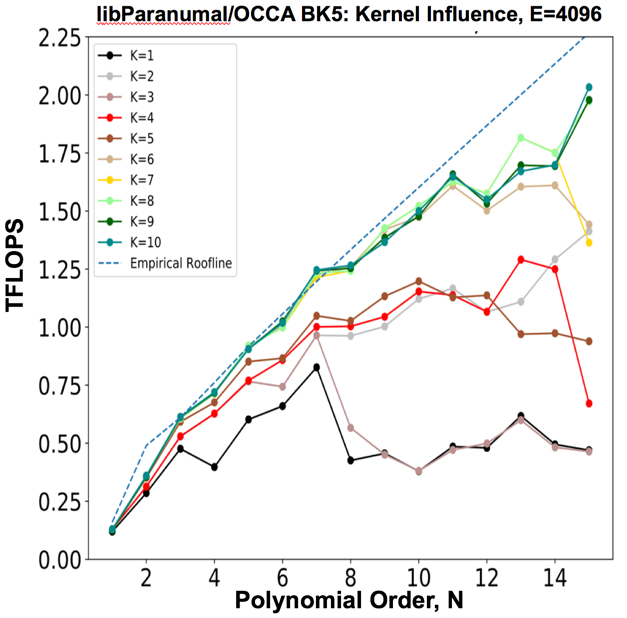
\includegraphics[width=0.94\textwidth]{figs/libp_kernels.png}
\caption{\label{fig:roof}\small{
libParanumal Poisson-operator kernel development (iterations $K=1,\dots,10$)
vs.  polynomial order, $N$   \cite{ceed_bp_paper_2020}.}}
\vspace{-0.8em}
\end{wrapfigure}
\noindent{\bf Parallel Performance.}
NekRS has been developed in close collaboration with the libParanumal project
\cite{warburton2019,ChalmersKarakusAustinSwirydowiczWarburton2020,streamParanumal2020},
which provides high-performance kernels for high-order methods on GPUs.  The
kernels are written in OCCA to abstract between different parallel languages
such as OpenCL, CUDA, and HIP. OCCA allows developers to implement parallel
kernel code in a slightly decorated C++ language, OKL.  At runtime, the user
can specify which parallel programming model to target, after which OCCA
translates the OKL source code into the desired target language and
Just-In-Time (JIT) compiles kernels for the user's target hardware
architecture.  In the OKL language, parallel loops and variables in special
memory spaces are described with simple attributes. For example, iterations of
nested parallel {\em for} loops in the kernel are annotated with
\texttt{@outer} and \texttt{@inner} to describe how they are to be mapped to a
grid of work-item and work-groups in OpenCL or threads and thread-blocks in
CUDA and HIP. All iterations that are annotated with \texttt{@outer} or
\texttt{@inner} are assumed to be free of loop carried dependencies.
The OCCA-based libParanumal kernels
typically saturate the roofline on the NVIDIA GPUs, as illustrated
in Fig. \ref{fig:roof}, where we see that the local Poisson kernel
(without parallel communication) realizes 1.25 TFLOPS FP64 for polynomial
order $N=7$ on a single V100 of Summit \cite{ceed_bp_paper_2020}.





Through extensive performance tuning including covering communication with
computation, use of mixed precision in preconditioners to reduce
injection-bandwidth pressure, improved preconditioners, projection-based
initial guesses \cite{fisc98}, and run-time optimized
communication strategies that select between GPU-direct, GPU-packed+host-based,
or pure host-based communication, we have made significant strides in delivering
performance for NekRS \cite{nekrs}.  On Summit, NekRS is significantly faster at
its strong-scale limit ($n/P \approx $2.1M, where $P$ is the number of V100s)
than Nek5000 is on Mira at its strong-scale limit ($n/P \approx 4000$, where $P$
is the number of ranks in -c32 mode).\footnote{In both cases, we identify the
strong-scale limit as the value of $n/P$ where the code realizes $\approx$80\%
efficiency, which is commensurate with production runs and therefore our target
performance-design-point.}  Production runs at the strong-scale limit realize
about 0.5--1.0 seconds per step for Nek5000 on Mira, while NekRS typically
requires only 0.1--0.4 seconds per step on Summit.  Moreover, production
Nek5000 runs on all or half of Mira were limited to about 15 million elements
($n \approx 5$B), whereas 100-million-element runs with $n \approx 50$--75
billion are readily accessible on Summit with NekRS operating at its
strong-scale (i.e., {\em fast}) limit.
Table \ref{tab:mira} compares the Nek5000/NekRS Mira/Summit
performance for DNS of a 1.1B-point rod-bundle simulation with a detailed
spacer grid geometry.  The Mira data point is at its strong-scale limit
of $n/P \approx 4000$.  The Summit scaling indicates 80\%
efficiency is realized at $n/P \approx 2.1M$.  At these representative
points, NekRS/Summit is about 4.5 times faster than Nek5000/Mira. \\


%%%%%%%%%%%%%%%%%%%%%%%%%%%%%%%%%%%%%%%%%%%%%%%%%%%%%%%%%%%%%%%%%%%%%%%
\begin{table*}[t]
\newcolumntype{?}[1]{!{\vrule width #1}}
  \footnotesize

  \begin{center} \begin{tabular}{|l|l|c|r|r|r|r|r|r|r|}
  \hline
  \multicolumn{10}{|c|}{{\bf Spacer-Grid DNS Performance on Mira vs. Summit, $E=3235953$, $N=7$, $n=1.10B$}} \\
  \hline
  \hline
  System & Code      & Device & Node & Rank & R/N & $E$/Rank & $n$/Rank &  $t_{step} (s) $ &  Eff  \\
  \hline
  \hline
   Mira  &Nek5000&CPU &  8192 &262144 & 32 &  12   &  4116   &  6.90e-01 & 100  \\
  \hline
  \hline
%%%%%%%%
%OLD data&       &    &   38  & 1596  & 42 &  2027 & 695446  &  1.06e+01 & 100  \\
%%%%%%%%
         &       &    &   38  & 1596  &  42 & 2027  & 695446 &  1.68e+01 & 100 \\
  Summit &Nek5000&CPU &   76  & 3192  &  42 & 1013  & 347723 &  0.50e+01 & 106 \\
         &       &    &  152  & 6384  &  42 & 506   & 173861 &  0.23e+01 & 114 \\
         &       &    &  304  &12768  &  42 & 253   &  86930 &  0.11e+01 & 120 \\ \hline \hline
         &       &    &   38  & 228   &   6 &  14193&  4.8M  &  2.75e-01 & 100 \\
  Summit & NekRS &GPU &   60  & 360   &   6 &  8988 &  3.0M  &  1.92e-01 &  90 \\
         &       &    &   76  & 456   &   6 &  7096 &  2.4M  &  1.64e-01 &  84 \\
         &       &    &   98  & 588   &   6 &  5503 &  1.8M  &  1.39e-01 &  77 \\
  \hline
  \multicolumn{10}{ c }{{}} \vspace*{-.4in}
  \end{tabular}
  \end{center}
\caption{\label{tab:mira}\small
Spacer-Grid performance on Mira (Nek5000), Summit CPU (Nek5000), and Summit GPU
(NekRS).  $t_{step}$ is the average wall-time in seconds over 100 timesteps with $\dt$= 6.e-5 (CFL=1.706) at $Re_D=14000$
with pressure tol= 1.e-05 and velocity tol= 5.e-12. R/N is the number of ranks per node. }
\end{table*}
%%%%%%%%%%%%%%%%%%%%%%%%%%%%%%%%%%%%%%%%%%%%%%%%%%%%%%%%%%%%%%%%%%%%%%%



%%%%%%%%%%%%%%%%%%%%%%%%%%%%%%%%%%%%%%%%%%%%%%%%%%%%%%%%%%%%%%%%%%%%%%%

 \begin{table}[b]
 \footnotesize
 \begin{tabular}{|r|r|r|c|c|c|r|}
  \hline
% \multicolumn{7}{|c|}{{\bf Rod Bundle Strong Scale: $v_i=3$, $p_i=2$, $E= 175618000$, $N=7$, $n=60B$}}\\
% \multicolumn{7}{|c|}{{\bf NekRS Strong Scale:  Rod-Bundle,  200 Steps}}\\
  \multicolumn{7}{|c|}{{\bf NekRS Strong Scale:  Rod-Bundle}}\\
  \hline
 Node & GPU   & $E$ & $n$ & $n/P$ & $t_{\rm step} (s) $ & Eff \\
 \hline
 1810 &10860 &  175M & 60B &5.5M &1.85e-01 & 100  \\
 2536 &15216 &  175M & 60B &3.9M &1.51e-01 &  87  \\
 3620 &21720 &  175M & 60B &2.7M &1.12e-01 &  82  \\
 4180 &25080 &  175M & 60B &2.4M &1.12e-01 &  71  \\
 4608 &27648 &  175M & 60B &2.1M &1.03e-01 &  70  \\
      &      &       &     &     &         &      \\
  \hline
 \end{tabular}
 \vspace*{.3in}
 \begin{tabular}{|c|c|c|c|c|c|r|}
  \hline
% \multicolumn{7}{|c|}{{\bf Rod Bundle Strong Scale: $v_i=3$, $p_i=2$, $E= 175618000$, $N=7$, $n=60B$}}\\
% \multicolumn{7}{|c|}{{\bf NekRS Weak Scale: Rod-Bundle, 200 Steps}}\\
  \multicolumn{7}{|c|}{{\bf NekRS Weak Scale: Rod-Bundle}}\\
  \hline
 Node & GPU &  $E$ & $n$      &  $n/P$& $t_{\rm step}(s)$ & Eff  \\
 \hline
 87   & 522   & 3M        & 1.1B  &  2.1M  & 8.57e-02  & 100   \\% 100   \\
 320  & 1920  & 12M       & 4.1B  &  2.1M  & 8.67e-02  & 99    \\% 98.7  \\
 800  & 4800  & 30M       & 10B   &  2.1M  & 9.11e-02  & 94    \\% 94.0  \\
 1600 & 9600  & 60M       & 20B   &  2.1M  & 9.33e-02  & 92    \\% 91.8  \\
 3200 & 19200 & 121M      & 41B   &  2.1M  & 9.71e-02  & 88    \\% 88.2  \\
 4608 & 27648 & 175M      & 60B   &  2.1M  & 1.03e-01  & 83    \\% 82.5  \\
 \hline
 \end{tabular}
 \caption{\small\label{rod-strong-weak} NekRS full-scale performance on Summit.}
%\caption{\label{rod-strong-weak}
%   NekRS strong and weak scaling for rod bundle simulations.
%   $n/P$: number of grid points per gpu,
%   $E/P$: number of elements per gpu,
%   $t_{\rm step}$: average wall time for 101--200 steps,
%   and Eff: efficiency.
%   BDF3+EXT3 is used for timestepping with $\Delta t=$ 3e-4,
%   corresponding to CFL=0.54.
%  }
\end{table}
%%%%%%%%%%%%%%%%%%%%%%%%%%%%%%%%%%%%%%%%%%%%%%%%%%%%%%%%%%%%%%%%%%%%%%%%%%

%% NEK: strong/weak rod1717
\noindent{\bf Strong- and Weak-Scaling.}
Table~\ref{rod-strong-weak} demonstrates NekRS scaling on Summit for a
$17 \times 17$ rod-bundle configuration, averaged over 100 timesteps
using 3rd-order timestepping with a Courant number of CFL=0.54.
In this case, 80\% strong-scale efficiency is realized for
$n_{0.8} = n/P \approx 2.6$M.  The weak-scale study was conducted at a
challenging value of $n/P = $2.1M $< n_{0.8}$ and sustains $> 80\%$
efficiency out to all of Summit---over a 50-fold increase in processor count.
%%%% $n/P$: number of grid points per gpu,
%%%% $E/P$: number of elements per gpu, $t_{\rm step}$: average wall time for
%%%% 101--200 steps, and Eff: efficiency.  BDF3+EXT3 is used for timestepping with
%%%% $\Delta t=$ 3e-4, corresponding to CFL=0.54.

%% NEK: pebbles
%% fluid mesh comprising $E = 98782067$
%% is the full core for the pebble bed reactor, which
%% has 352,625 spherical pebbles and a fluid mesh comprising $E = 98782067$
%% elements of order $N=8$ ($n\approx 51B$).

%% NEK: single rod on advaned arch
Table~\ref{peb352k-strong} shows strong-scaling for the 352,625-pebble reactor
configuration of Fig. 1 (right), which is representative of the type of flow
compexity anticipated in the proposed work.  Here, the pressure Poisson
problem is challenged and requires an average of 7.2 iterations per step
for this $n=51$B gridpoint problem ($E$=98M, $N$=8).  The Courant number
is CFL $\approx$ 4.  For this case, the strong-scale limit is $n_{0.8}\approx 1.9$M.
Finally, in anticipation of running on Frontier, we present in
Table~\ref{singlerod} single-GPU results for NekRS on the AMD MI100.  These
results are enabled by the portability of OCCA, which has support for a HIP
back-end.  Without tuning, NekRS is only about 20\% slower on the MI100 than on
the V100.   We anticipate improvements in this performance with MI100-oriented
kernels.
For point of reference, we also include results for the NVIDIA
A100, which shows a 1.6 speed-up over the V100.
%%%% Table~\ref{singlerod} demonstrates NekRS performance on a single GPU for single
%%%% rod simulations for 500 steps and the averaged timing per step, $t_{step}$, is
%%%% measured in seconds for 101-500 steps.  R is the ratio of $t_{step}$ to Summit
%%%% V100.  The timestep size is $\Delta t$=1.2e-03 (CFL=7.3).  Characteristic-based
%%%% BDF2 with 1 substeps is used for timestepping.  Tolerances for pressure and
%%%% velocity are  1e-4 and 1e-6, respectively.


%%%%%%%%%%%%%%%%%%%%%%%%%%%%%%%%%%%%%%%%%%%%%%%%%%%%%%%%%%%%%%%%%%%%%%%

%\begin{table}[!t]
%\newcolumntype{?}[1]{!{\vrule width #1}}
%  \footnotesize
%
%  \begin{center} \begin{tabular}{|l|l|c|r|r|r|c|r|}
%  \hline
%  \multicolumn{8}{|c|}{{\bf DNS $5\times 5$, Performance on Mira vs. Summit, $E=8387008$, $N=7$, $n=2.87B$}} \\
%  \hline
%  System & Code & Device & Node & Rank &  $n$/Rank &  $t_{step} (s) $ & Eff  \\
%  \hline
%  \hline
%  Mira    & Nek5000& CPU&    8192 &262144 &  10973   &7.00e-01 &  100  \\
%  \hline
%  \hline
%          &        &    &   175   & 7350   &  391393  &3.97e+00 &  100  \\
%   Summit & Nek5000& CPU&   1152  & 48384  &  59456   &9.51e-01 &   63  \\
%          &        &    &   2304  & 96768  &  29728   &7.30e-01 &   41  \\
%  \hline
%  \hline
%          &        &    &  87   &  522   &   5.5M &  2.30e-01 &  100   \\
%  Summit  & NekRS  & GPU& 120   &  720   &   3.9M &  1.83e-01 &  91    \\
%          &        &    & 160   &  960   &   2.9M &  1.49e-01 &  84    \\
%          &        &    & 220   & 1320   &   2.1M &  1.27e-01 &  71    \\
%  \hline
%  \end{tabular}
%  \end{center}
%  \caption{\label{dns-strong}Performance on Mira and Summit.}
%%\caption{\label{dns-strong} Performance on Mira (Nek5000) vs. Summit CPU (Nek5000) and GPU (NekRS).
%%Timings are in seconds for the wall time per step, $t_{step}$.
%%{\bf DNS $5\times5$}: 400 timesteps over simulation time interval [59.71, 59.78]
%% with $\dt$= 1.9e-04 (CFL=0.32) at $Re_D=19000$.  BDF2+EXT2. }
%\end{table}
%%%%%%%%%%%%%%%%%%%%%%%%%%%%%%%%%%%%%%%%%%%%%%%%%%%%%%%%%%%%%%%%%%%%%%%%%%%




%%%%%%%%%%%%%%%%%%%%%%%%%%%%%%%%%%%%%%%%%%%%%%%%%%%%%%%%%%%%%%%%%%%%%%%%%%
\begin{table}
\footnotesize
\begin{center}
\begin{tabular}{|r|r|r|c|c|c|r|}
  \hline
  \multicolumn{7}{|c|}{{\bf NekRS Srong Scale: 352K pebbles}, $E=98M$, $n=50B$}\\
% \multicolumn{7}{|c|}{Re=500, 2.e-3, 9, 13, 4.e-4, TOMBO2, 1, T, 8, F, CHEBY+JAC, 851}\\
% \multicolumn{7}{|c|}{{\bf $N=8$, $N_q=11$, $\Delta t=$ 8.e-4, $L=30$, 2-Cheb-ASM:8641}}\\
  \hline
  Node & GPU  & $n/P$ &  $v_i$ & $p_i$ & $t_{\rm step}(s)$ & Eff \\
  \hline
% 1536   &  9216  &   5.4M   &  -   &   -  &    -   &      -       \\% MEM GB  \\
  2304   &  13824 &   3.6M   &   5.7&   7.2&    .55 &    100       \\% 15.1    \\
  3072   &  18432 &   2.7M   &   5.7&   7.2&    .56 &    74        \\% 10.8    \\
  3840   &  23040 &   2.1M   &   5.7&   7.2&    .39 &    85        \\% 9.57    \\
  4608   &  27648 &   1.8M   &   5.7&   7.2&    .36 &    76        \\% 8.04    \\
 \hline
 \end{tabular}
\end{center}
 \caption{\small\label{peb352k-strong} NekRS full-core pebble-bed reactor, full-scale simulation on Summit.}
\end{table}
%%%%%%%%%%%%%%%%%%%%%%%%%%%%%%%%%%%%%%%%%%%%%%%%%%%%%%%%%%%%%%%%%%%%%%%%%%







 %%%%%%%%%%%%%%%%%%%%%%%%%%%%%%%%%%%%%%%%%%%%%%%%%%%%%%%%%%%%%%%%%%%%%%%%%
 \begin{table}[!t]
  \footnotesize
  \begin{center}
  \begin{tabular}{|l|l|l|c|c|c|c|}
  \hline
  \multicolumn{7}{|c|}{{\bf NekRS Single GPU Performance, $E=7168$, $N=7$, $n=2.4M$, $Re=5000$}} \\
  \hline
   system   & device &   API &  $t_{500}$ (s)    &   $t_{100}$  (s)  &   $t_{step}$ (s) & R \\
  \hline
    OLCF Summit   & NVIDIA V100  &  CUDA   &    4.089e+01  &  9.018e+00 &  0.0795 & 1.00   \\
    ALCF ThetaGPU & NVIDIA A100  &  CUDA   &    2.503e+01  &  5.587e+00 &  0.0485 & 0.61   \\
    OLCF Spock    & AMD MI100    &  HIP    &    5.007e+01  &  1.103e+01 &  0.0975 & 1.22   \\
    HPE Tulip     & AMD MI100    &  HIP    &    4.870e+01  &  1.060e+01 &  0.0953 & 1.19   \\
  \hline
  \end{tabular}
  \end{center}
  \caption{\small\label{singlerod} NekRS single GPU performance on advanced architectures.}
 %\caption{\label{singlerod} NekRS performance on a single GPU.
 % Simulations are performed for 500 steps and the averaged timing per step, $t_{step}$,
 % is measured in seconds for 101-500 steps. R is the ratio of $t_{step}$ to Summit V100.
 % Different versions of ROCm are used for MI100.
 % The timestep size is $\Delta t$=1.2e-03 (CFL=7.3).
 % Characteristic-based BDF2 with 1 substeps is used for timestepping.
 % Tolerances for pressure and velocity are  1e-4 and 1e-6, respectively.
 % }
 \end{table}
%%%%%%%%%%%%%%%%%%%%%%%%%%%%%%%%%%%%%%%%%%%%%%%%%%%%%%%%%%%%%%%%%%%%%%%%%


\noindent{\bf Project Workflow and I/O.}
The scale of the proposed problems on Summit and Frontier is signifcantly
larger than that of prior production runs on Mira.  For example, full-core
simulations of the pebble bed reactor  ($n$=50B) on all of Summit generate
single snapshot files of 1.4 TB, each, with 32 bit words.  Using MPI I/O, these
files are written in 40 seconds (32 GB/sec) for simulations that take about 0.4
seconds per step, which is tolerable.   Visualization and file movement,
however, are quite painful and we have had to develop specialized subsampling
techniques that collect only the ``visible'' elements to make image rendering
feasible.  We envision that compression techniques based on spectral (Legendre)
data representations will be useful for reducing file sizes; compression ratios
of up to 40:1 have been reported for this class of problems when applied to
Nek5000 \cite{otero18}.  Additionally, we are able to use Nek5000/RS to perform
all of the data analysis, at scale.  Both codes collect statistics (e.g., mean,
RMS, and cross-correlations) for velocity and temperature at runtime and
extensive turbulent-statistics post-processing utilities are available for
Nek5000 that are compatible with NekRS.

Another concern is construction and use of very large meshes.  The record
for Nek5000 on Mira was 15M elements.  We have recently extended Nek5000/RS
to support over 1B elements ($n$=216B).   This extension required promoting
several arrays to support int8 indexing during problem-setup.  (These
are arrays that are used to identify face-face and edge-edge connections
between elements---the array sizes scale as $E/P$ and are thus fully
scalable.)   Fortunately, for mesh construction, we can use many of the
available FEM tools because the number of elements required for the SEM
is two orders of magnitude smaller than that required for low-order FEM
simulations at the same resolution.
For mesh partitioning, we have recently developed parallel domain partitioners,
parRCB and parRSB, that couple with Nek5000/RS.  parRCB uses recursive
coordinate bisection and parRSB uses recursive spectral bisection
\cite{pothen90}.  We use parRCB as a precursor decomposition for parRSB in
order to minimize the data volume during the communication-intensive Lanzcos
iterations that are used to find the Fiedler vector required for RSB.



\vspace{-.25in}
\subsection{Developmental Work}
\vspace{-.2in}

% For the computational approach described above, describe what, if any,
% development work has been carried out to-date, especially on the architecture
% of the requested resource. Describe what development work will be executed
% during the proposed INCITE campaign and when it will be executed. Provide an
% estimate of the computational resources required for this work. If
% applicable, identify the milestones and production activities in Section
% 2.3.i that are dependent on the developmental work and provide a plan for
% validating this developmental work.

NekRS has been demonstrated at the capability computing level on Summit
for full- and partial-core reactor systems with excellent parallel performance.
No additional developmental work is required for the proposed research -- our
team is immediately ready to conduct the high-impact science described.

\clearpage
\vspace{-.15in}
\section{REFERENCES}
\vspace{-.15in}

%References are optional and may be structured in accordance with any style. They {\bf \em {do}} count toward the 15-page limit.


\renewcommand{\section}[2]{}%	No 'References' title
%\renewcommand{\chapter}[2]{}% for other classes


\bibliographystyle{ieeetr}
\bibliography{references,ref_nt,emmd,main}

\end{document}
